\section{\texttt{shiny}}

% ----------------------------------------------------------------------

\subsection{Descrição}

\begin{frame}

  \texttt{shiny} torna incrivelmente fácil construir aplicações web
  interativas com o R. Ligação entre \emph{inputs} e \emph{outputs} que
  são reativos e um conjunto extenso de \emph{widgets} permitem
  construir interfaces atraentes, responsivas e poderosas para a web com
  esforço mínimo.

  \begin{itemize}
  \item Autores: Winston Chang, Joe Cheng, JJ Allaire, Yihui Xie,
    Jonathan McPherson, e muitos contribuidores
  \item Lançamento: 01-Dec-2012
  \item Versão: 0.12.1
  \item URL:
    \url{http://cran.r-project.org/web/packages/shiny/index.html},
    \url{http://shiny.rstudio.com/}
  \end{itemize}

\end{frame}

% ----------------------------------------------------------------------

\subsection{Como usar}

\begin{frame}
  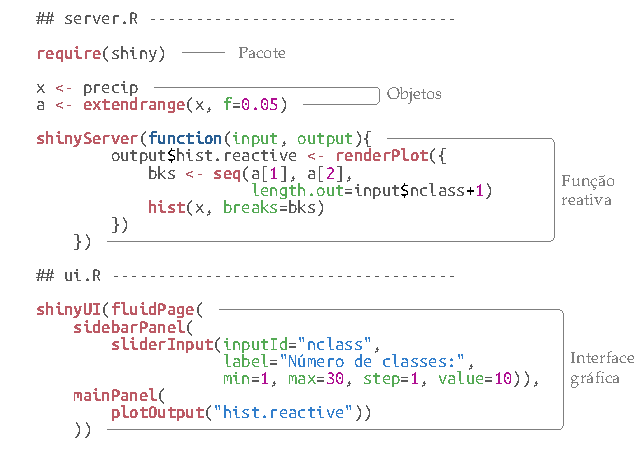
\includegraphics[scale=0.98]{./tikz/hist_slider_shiny-1.pdf}
\end{frame}

\begin{frame}
  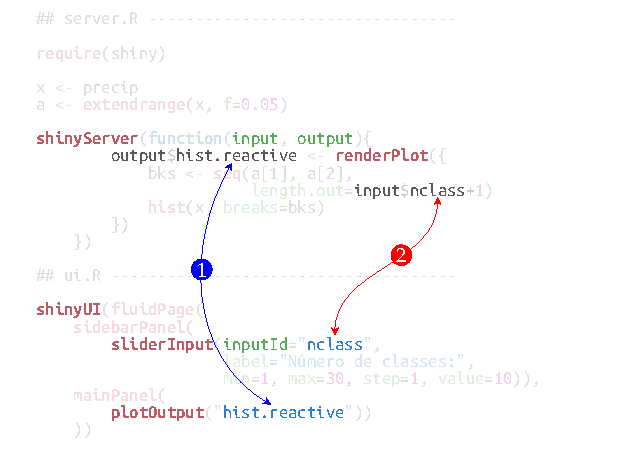
\includegraphics[scale=0.98]{./tikz/hist_slider_shiny-2.pdf}
\end{frame}

\frame{
  \begin{center}
    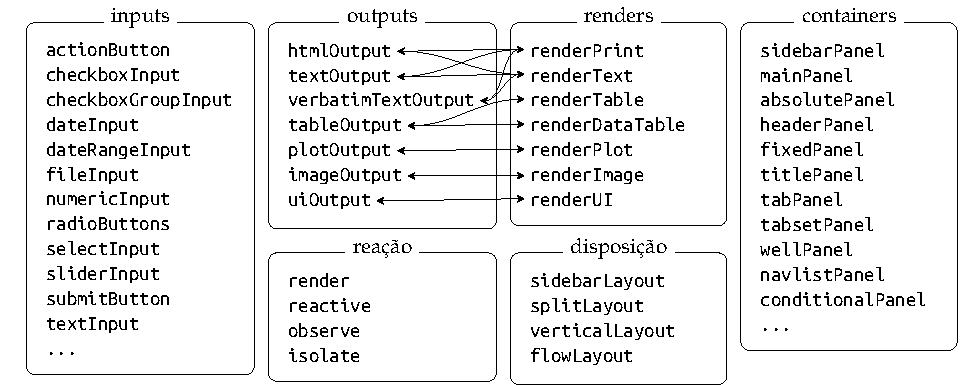
\includegraphics[width=0.98\linewidth]{./tikz/shiny_fun.pdf}
  \end{center}
}

\frame{
  \begin{center}
    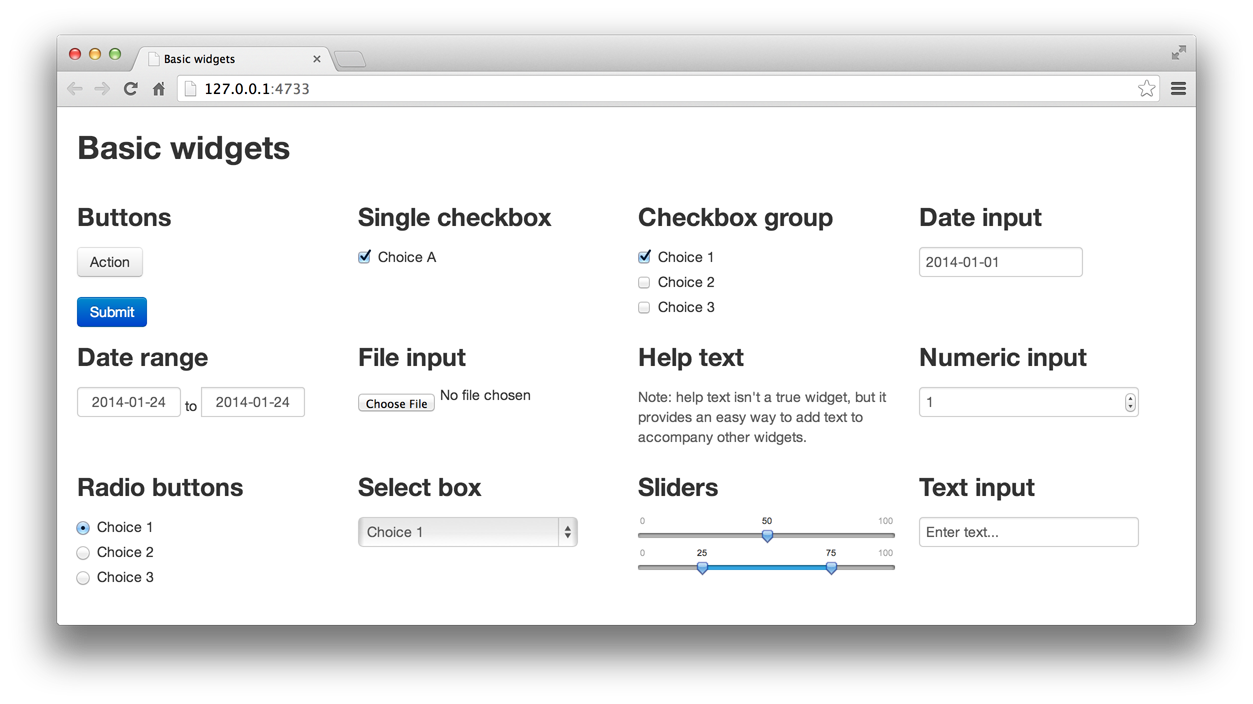
\includegraphics[width=0.98\linewidth]{./images/shiny-widgets.png}
  \end{center}
}

\frame{
  \begin{center}
    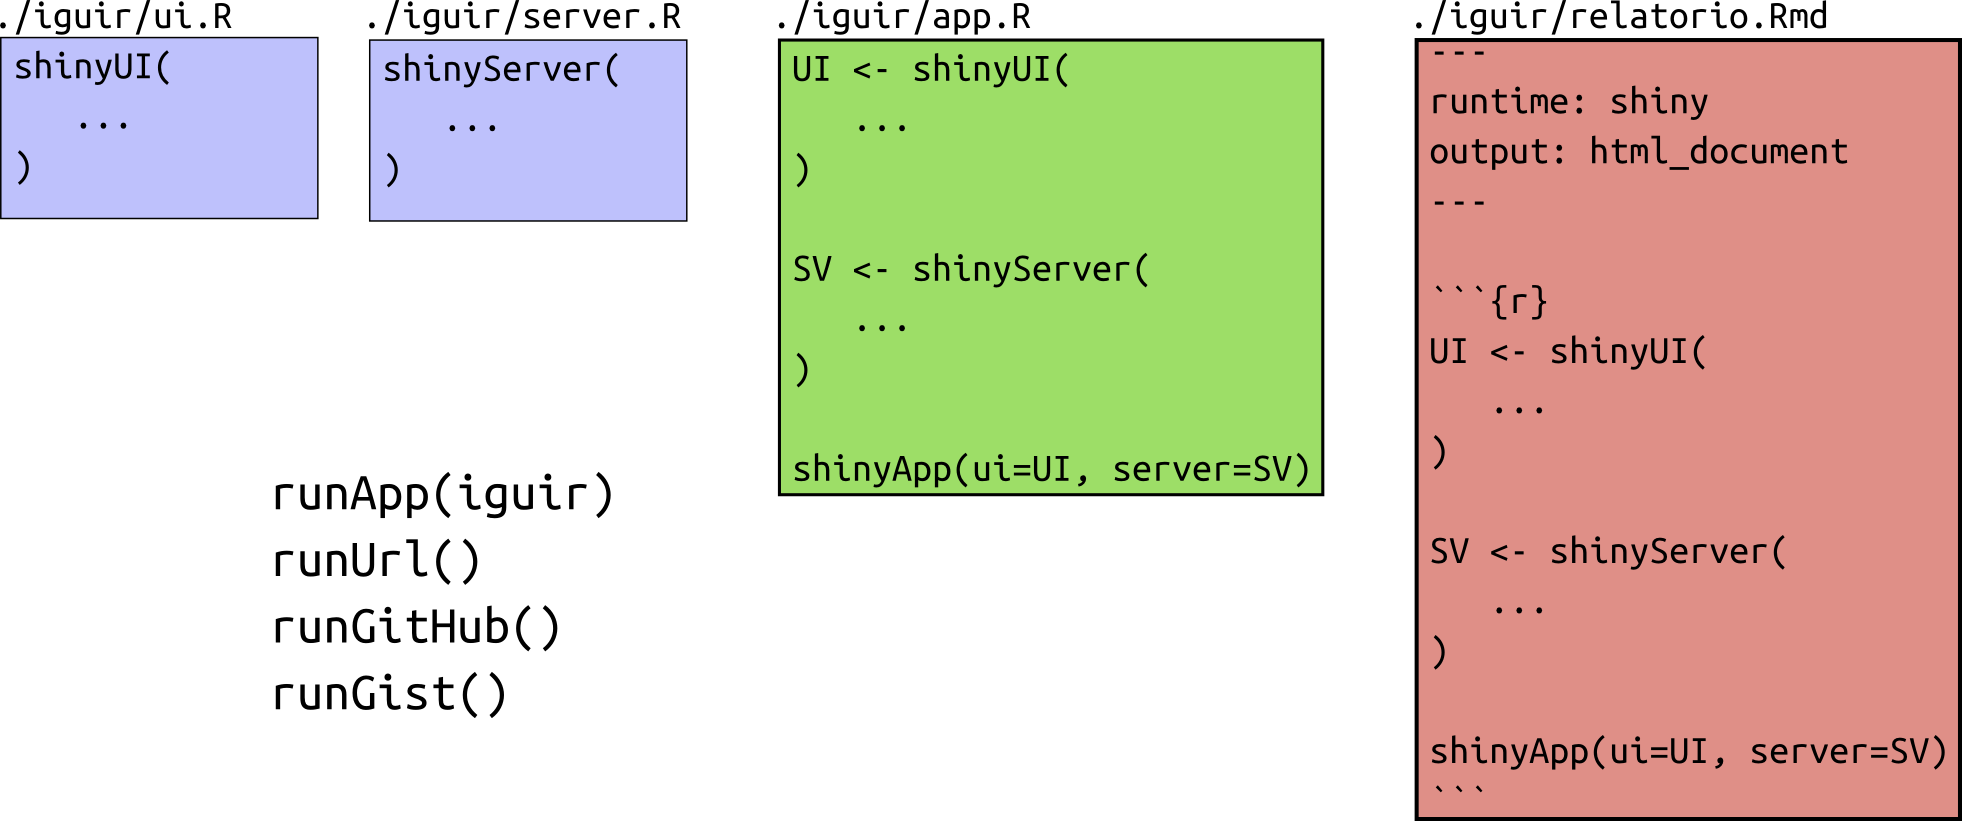
\includegraphics[width=0.98\linewidth]{./images/shiny_docs.png}
  \end{center}
}

\begin{frame}
  \begin{itemize}
  \item Criar aplicações com GUI (abrem no navegador);
  \item Produzir relatórios de análises web interativos;
  \item Não é necessário conhecimento de HTML, CSS ou JavaScript;
  \item Públicar aplicações na web
    \begin{itemize}
    \item \url{http://www.shinyapps.io/}
    \item Servidor Shiny próprio
      (\href{http://shiny.leg.ufpr.br/iguir/list/}{Shiny LEG \& PET})
    \end{itemize}
  \item O público não precisa ter/saber o R.
  \end{itemize}
\end{frame}

% ----------------------------------------------------------------------

\subsection{Exemplos}

\begin{frame}
  Praticando:
  \begin{enumerate}
  \item \href{run:./R/shiny/app.R}{R Script shiny}
  \item \href{run:./R/shiny/shiny}{Diretório shiny}
  \end{enumerate}

  \vspace{0.5cm} Algumas galerias de aplicações em shiny:

  \begin{itemize}
  \item \href{http://shiny.leg.ufpr.br/iguir/list/}{Galeria shiny iguiR}
  \item \href{http://shiny.leg.ufpr.br/walmes/list/}{Galeria shiny do
      Walmes}
  \item \href{http://shiny.rstudio.com/gallery/}{Galeria Shiny Oficial}
  \item \href{http://www.showmeshiny.com/}{Galeria Shiny}
  \end{itemize}
  
\end{frame}

\begin{frame}
  Algumas aplicações em \texttt{shiny}:
  \begin{itemize}
  \item \href{http://www.stat.cmu.edu:3838/hseltman/LogReg/}{Logistic
      Regression Residual Analysis}
  \item \href{https://ilame.shinyapps.io/Test3}{Body Mass Index
      Calculation Tool}
  \item
    \href{https://hseltman.shinyapps.io/QuantileNormal}{Investigation of
      Quantile-Normal Plots Through Simulation}
  \item
    \href{http://www.stat.cmu.edu:3838/hseltman/PrePost/}{
      Pre-test/Post-test Simulation}
  \item
    \href{http://www.stat.cmu.edu:3838/hseltman/TransferFunctions/}{
      Explore Transfer Functions}
  \item
    \href{http://nbcgib.uesc.br/lec/avale-es/amb-virtual/inferencia/anava}{
      Fundamentos da análise de variância}
  \item
    \href{http://nbcgib.uesc.br/lec/avale-es/amb-virtual/probabilidade/con-frequentista}{
      Conceito frequentista de probabilidade}
  \end{itemize}

\end{frame}
